\documentclass{cmspaper}
\def\RCS$#1: #2 ${\expandafter\def\csname RCS#1\endcsname{#2}}
\RCS$Revision: 1.2 $
\RCS$Date: 2004/05/27 12:46:28 $

\usepackage{graphicx}

\begin{document}
\begin{titlepage}
  \whitepaper
  \date{Revision \RCSRevision, \RCSDate}
  \title{CMS Data Handling Overview}

  \begin{Authlist}
    Tim~Barrass, Simon~Metson\Instfoot{bristol}{University of Bristol, Bristol, UK}
    Lassi~A.~Tuura\Instfoot{neu}{Northeastern University, Boston, USA}
  \end{Authlist}

  \begin{abstract}
    This white paper presents an overview of the CMS data handling system.
  \end{abstract} 

  \note{DRAFT version}
\end{titlepage}

\setcounter{page}{2}

\section{Context}
During a recent data challenge CMS developed and tested a file transfer management structure, drawing on aspects of blackboard and multi-agent system design. Persistent, stateful distributed agents were deployed at a number of geographically distributed sites, and handled point to point propagation of files through the system. Communication between agents (typically announcing the presence of files at some point in the system) was prohibited by design; propagation of information through the agent system required the agents to post information at a central "blackboard". This blackboard was implemented in Oracle and named the Transfer Management Database, or TMDB. 

This architecture enabled us to maintain a coherent picture of system state in a central location, making it relatively trivial to diagnose and solve problems. It also meant that agent development was characterised by short timescales (the agents could be implemented in a local language of choice), and simplicity (as communication and coordination between agents was prohbited, and interaction with the TMDB was possible using any of a number of Oracle access libraries).

The first system was characterised by a single data source. Files were allocated to destinations and passed through a defined network topology (a hierarchy of sites) to those destinations, where the files were migrated to mass storage and/or submitted to realtime analysis.

The key change in version 2 is the provision for multiple data sources. We manage this change by noting that in version 1, transfer agents were logically equivalent to internet routers- routes were effectively hard-coded into the agents.  In the next version we draw on established internet routing algorithms to maintain a view of routes (and distances) through the system.

This entails a re-expression of information in the TMDB: replicas now have a generic source rather than a single source. A control agent (similar in role to a replica manager in other schemes) uses global policy to allocate files to a set of destinations.  Originally, this control agent monitored end to end system performance and could make failover decisions if sections of the network became unavailable. The control agent no longer handles failover- this can be handled, if required, by the routing algorithm. Instead, it just allocates files to a set of destinations, ensuring that all files have some destination.

The role of the system we present here is thus very tightly focused: source agents make files available to distribution by posting information in the TMDB. Once the files are allocated according to some global policy, the system handles the propagation of files through the system to a set of destinations.

[The system is beginning to separate into layers: the transfer management layer is what we describe here. However, another layer (replica management) is emerging. Both layers communicate through the TMDB- some structures that are replica-management focused are posited for the TMDB in this version, i.e. the file destinations table...] 

\section{Introduction}
Version 2 draws on our experience of managing agents with version 1. We found that at each site a ``manager'' process was required- a simple cron job in most cases- that could bring agents back up when they died.  In this document the term ``node'' is used to refer to a coherent (local) unit of agents, managers and buffers.

Nodes (fig. \ref{nodes}) are generically seen as logically equivalent to internet routers\footnote{Some dedicated nodes will only manage global, or resource amangement agents, like the configuration agent.}; they register with other nodes (routing agents register their node with another node in a global routing table) and share information about known routes to other nodes.  The routing of files around the network is governed by a modified implementation of the Routing Internet Protocol.

In this new structure failover can either be ignored, or handled by the nodes rather than by a global configuration agent (the config agent now only need to assign guids to destinations).  The routing algorithm incorporates a simple method of handling failover and recovery, in which failover becomes more dynamic re-establishment of routes rather than a route defined when a file enters distribution.

When a transfer agent wants to notify other agents that it has made a new file available (after transfer), it can determine where to advertise the file by examining file destination and global routing information in the TMDB to determine the shortest path to those destinations.

Agents in this new system can be categorised as data source agents, transfer agents, or as global agents (e.g. configuration agents- although only one configuration agent is necessary).

\section{Requirements of the system}
For version 2 our requirements come solely from production, and are:

\section{System architecture and data flow}
\subsection{Overall architecture}
As described above, a blackboard architecture is chosen as the basis for the system. Traditional blackboards, however, often instantiate components wit specific tasks when triggered by certain events- the instantiated components are transient and stateless. In this system, the components actively taking part in distributing data are persistent and stateful agents. 

The blackboard in this case is an Oracle database, named the Transfer Management Database, or TMDB. All communication between agents is via the TMDB; there is a small, defined set of message forms possible, meaning that complex functionality is contained within the agents, and only simple, essential messages are shared (fig. \ref{sample-transfer}).

The agents run concurrently, and are not (in version 2) triggered by new data appearing in the TMDB.  All agents publish their state with each polling loop they make- agents that do not publish their state over a certain time period are thought to be down.

The distribution network is thought to be well defined, although the system is generic enough that a fully-connected network is possible. Our system requirements suggest a hierarchical or tiered network, with a single tier-0 site, and increasing numbers of tier-1 and tier 2 sites. The tier-0 and tier-1 sites will be fully-connected. Tier-2 sites will only be connected to a single tier-1 (fig. \ref{network}).

While in distribution files are thought to have some "value", which impacts the desired lifetime of replicas at each node in the system. This lifetime needs to be managed, or rather governed, by global policy\footnote{Some replicas will be of vital importance and exempt from local policy, while other replicas may be more expendable.}. In particular nodes can not delete replicas at will: it might be vital that copies of the file are kept in the system until they are, for example, made safe in at least two mass storage systems. This information is available in the TMDB, and focused buffer cleaning agents can coordinate in the solving of this deletion problem by exchanging information there. In doing this they can make use of local lifetime management mechanisms- e.g. pinning files on MSS stage disk, not marking files as voltile in SRM- but the overall control should remain with higher level agents.

\subsection{Transfer Management Database}
The Transfer Management Database is dealt with in a separate whitepaper. Basically, it's components are Lookup, Routing, File Bookkeeping, Transfer Queue/File State...

\subsection{Routing agents}
Routing agents are dealt with in a separate whitepaper. Basically-

\subsection{Data source (dropbox) agents}
publish availability (log), process drop (log)

\subsection{Global agents (basic resource management)}
publish availability,

\subsection{Transfer agents}
Transfer agents poll the TMDB for a list of guids newly advertised for them. They typically choose some subset of the guids, guided by "local" policy, presently hardcoded into the agent, to avoid e.g. excessive load on disk, etc. These guids are then queued and transferred, with the agent using some form of grid tool to make the transfer (version 2 will probably be using lcg-2 rm and globus-url-copy). The file catalogue is updated.

The agent then determines the final destination(s) of the file. Using the routing information, it determines which gateways to advertise these files for (i.e. which nodes are the next step in the chain) and posts messages in the TMDB for those gateway nodes \footnote{There are inefficiencies in this algorithm- for example, files may already exist at nodes for which they are advertised- thus the readvertisement of the file, and the unrequired attempt to transfer are unnecessary. These can be trivially avoided by noting that checking for file existence is quite straightforward, and the re-registration of information in the TMDB can be handled by Oracle mechanisms. See the routing white paper for more details.}.

\subsection{Buffer cleaning agents}
Strategies used by buffer cleaning agents will vary- these strategies will eventually need to be guided by policy, a subject which will need to be addressed in future versions of the system. Several strategies were used in version 1 agents. Simple cleaning agents were able to check if files had entered a safe state- i.e. been migrated to tape- at each of the destinations to which they were connected. Once safe, replicas at the intermediate nodes
could be cleared.

A more sophisticated strategy, emplyed at the tier-0, ranked local replicas based on age, number of replicas in tape storage, and number of replicas still present at intermediate stages. Replicas of low rank were deleted (actually migrated to tape store in this case and removed from disk).

\section{Future directions}
Policy: mostly tied into global/config/resource/replica management structure (layer above this). We need a sense of file value (like the ranking we already have), and how to redirect valuable files in flight if they get stuck, or need to be put into mass storage quickly. We need a generic statement of strategy which can guide these policies. We need policies a various granularities (file, dataset, site[T2,T1,T0], global) to determine how to react in given circumstances. Much of this can be hardcoded into the replica/resource management to start with, but can it be abstracted so that changing policies can be accounted for?

[Question of policy: We need a maximum number of hops associated with
a file before it times out and just needs to get placed in mass
storage anywhere? Can implement this if record node type info (or
maybe whether it has a mass store). Destination can be dynamically
changed by something monitoring files (global?) that can check whether
a file has reached it's maximum lifetime in distribution and just
needs to be sent straight to the closest mass store. For next
version?]

\clearpage
\begin{figure}
\centering
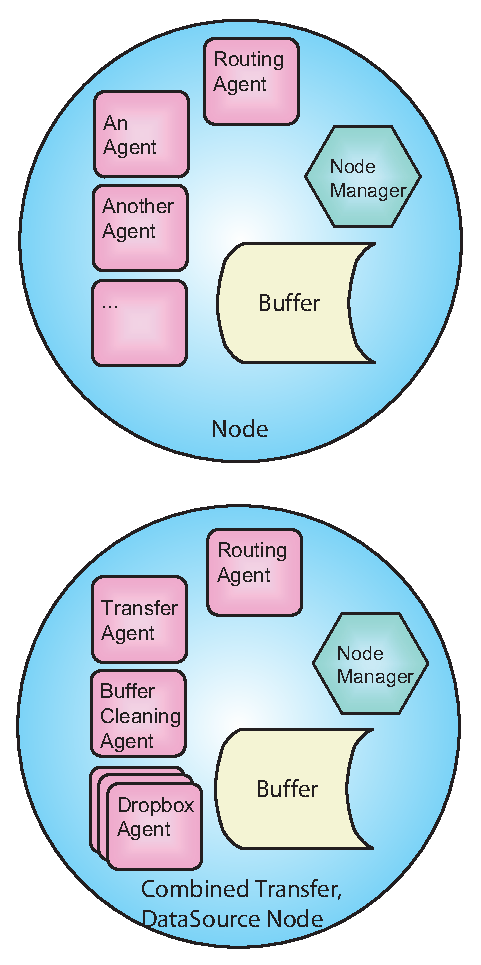
\includegraphics{nodes.eps}
\caption{Nodes are composed various components. A node manager (which keeps agents alive in this version) is always present. In addition, there will always be one or more agents. In nodes that act as routers, a routing agent will be present. Nodes that transfer files will have some form of buffer (SE, MSS...).}
\label{nodes}
\end{figure}

\clearpage
\begin{figure}
\centering
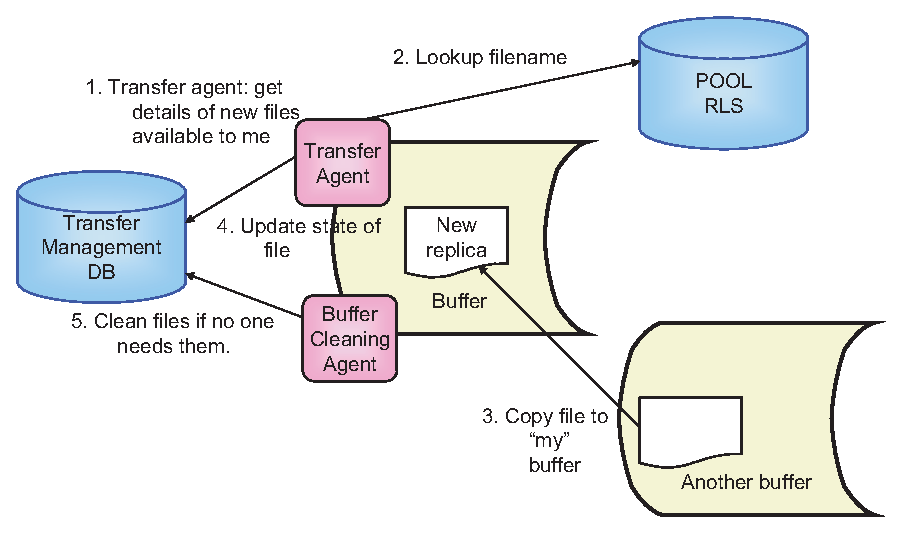
\includegraphics{sample-transfer.eps}
\caption{Few messages are exchanged between components in the system (shown here is a sample query for pending transfers, transfer, and clean). Queuing of pending transfers and so on are all handled within the agent.}
\label{sample-transfer}
\end{figure}

\clearpage
\begin{figure}
\centering
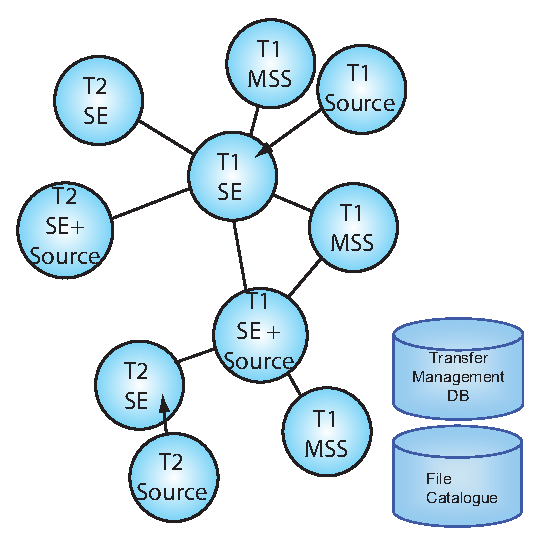
\includegraphics{network.eps}
\caption{The network is based on a tier structure, although for version 2 the nodes are equivalently weighted in terms of routing importance. Preferred routes are chosen by careful construction of network topology (i.e. mass storage nodes are placed on spurs from the main network, so files aren't routed through them on the way to other destinations.}
\label{network}
\end{figure}


\end{document}
